% This example An LaTeX document showing how to use the l3proj class to
% write your report. Use pdflatex and bibtex to process the file, creating 
% a PDF file as output (there is no need to use dvips when using pdflatex).

% Modified 

\documentclass{l3proj}
\begin{document}

\title{ESE1 Team Project Dissertation}

\author{Agnes Ola \\
        Ross James Gardiner \\
        Lorenzo Roccato \\
        Duncan Lowther \\
        Nawaf Al Lawati}

\date{6 April 2020}

\maketitle

\begin{abstract}

What follows is a case study of the construction of the NextSTEPS application using the agile software development process. This is a project by Team ESE1 for customer Sports Labs. Our product was created for the completion of the university module Team Project 3. 

Throughout this paper, we discuss the project itself, the customer, our delivered product and several reflections highlighting lessons learned during our work. 
%% The abstract goes here

\end{abstract}

%% Comment out this line if you do not wish to give consent for your
%% work to be distributed in electronic format.
\educationalconsent

\newpage
%==============================================================================
\section{Introduction}

This paper presents a case study of the NextSTEPS application and its constructing agile development process. NextSTEPS is team ESE1's evolutionary improvement on the STEPS (Sports Test Equip Performance Software) application. STEPS is a program for interacting with hardware designed to test sports playing surfaces. This hardware is the Advanced Artifical Athlete (AAA) \ref{fig:AAA}. The program signals the release of a powerful electromagnet and records information from an accelerometer. This is used to calculate metrics about the playing surface. The project involved a plethora of programming challenges, from low-level hardware interrogation to data visualisation techniques. The addition of hardware also makes our work unique, and brought an interesting flavour to our experience of the agile software process. 
\\
This paper first deals with our client, Sports Labs. We then discuss the requirement for the development of NextSTEPS and an overview of our final delivered product. 
\\
To document the learning experience of the team, we cover three reflections, Propagation of Early Design Decisions, Agile Testing for Hardware Dependant Software and Overly Ambitious Sprint Deliverables. Each reflection envelops a challenge the team had, the reasons for our shortcomings and how we can address them in the future. 
\\
To close, this paper includes several concluded learning outcomes attained by this work. 

\begin{figure}[h]
\label{fig:AAA}

\centering
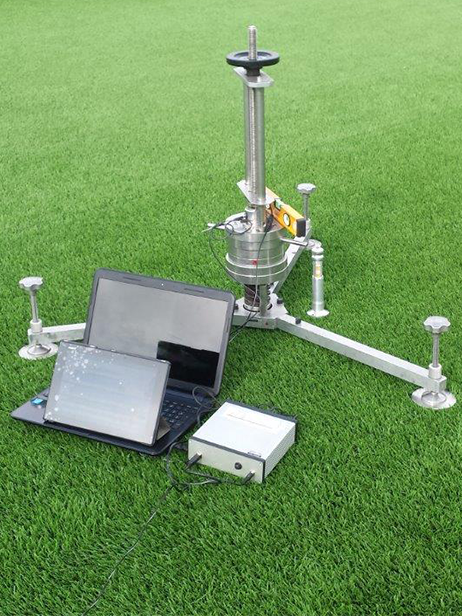
\includegraphics[width=0.5\textwidth]{./images/AAA+3.png}
\caption{Advanced Artificial Athlete (AAA) Hardware \cite{sportstestequip} }
\end{figure}

%==============================================================================
\section{Case Study Background}
\subsection{Our Client}
Sports Labs Ltd. is a Scottish company based in Livingston, West Lothian. The business operates within the sports surface testing and certifying industry as a service provider to many organisations requiring accreditation for their surfaces. Sports Labs work with many standards bodies such as the Fédération Internationale de Football Association (FIFA), International Hockey Federation (FIH) and World Rugby (WR) to certify more than 800 sports fields yearly in locations all over the globe. \\
In addition to field testing, the business  operates as a consultancy, a research and development team and a testing laboratory.\\
Our contact within the company, Chris Dyson is current manager for the company's R\&D team. He manages engineers from many disciplines (electrical, mechanical, biomedical) with a focus on developing apparatus test methods. In addition to this, Chris is involved in industrial projects with several universities besides the University of Glasgow including Edinburgh Napier and Glasgow Strathclyde.  
\subsection{Our Project}
We worked to improve one of the methods Sport Labs uses to certify sports surfaces - Determination of Shock Absorbtion (FIFA test method 04A). It consists of an accelerometer attached to a 20kg weight, suspended by an electromagnet. The weight is repeatedly dropped on a surface and the accelerometer data recorded. The shock absorption is calculated by comparing the maximum force on the test specimen with the reference force of impact on concrete\cite{fifa}. In other words, how soft the surface is compared to concrete after repeated compression. \\
The test apparatus consists of a tripod, an electromagnet, a weight, an accelerometer, a data acquisition unit (DAQ), a battery pack and software running on a Windows laptop with USB connection. The client is looking to make the test rig wireless to ease test execution, improve the DAQ (redesign the PCB to be more robust and compact) as well as get the test software running on Android so the technicians do not have to carry a laptop. These changes were quickly established to be out of scope of our project; however, we worked with these future directions in mind. \\
We agreed to redesign the legacy software solution. Our minimum viable product consisted of a program that runs on Windows, receives data from the DAQ over USB, receives calibration offset values, calculates the shock absobtion and displays the results on a graph. This program was to be written in Java for future cross platform compatibility. Our stretch goals were to implement wireless data transfer and port the application to Android platform.


\subsection{Our Software}
The software product we delivered is called "NextSTEPS" as a reference to its predecessor, "STEPS". It is written in Java and compiled into an executable, with the Sports Labs' logo as its icon. The program's prerequisites are InstaCAL drivers and Java version 1.9 or higher. The program does not require installation.

NextSTEPS meets the requirements agreed in the beginning of the project: it consists of a simple GUI, with options to choose calibration pre-sets, enable or disable the magnet on the Advanced Artificial Athlete hardware and start the test. Most of the window is taken up by the graph viewing panel that overlays consecutive tests. A panel on the bottom left corner records and averages the results of three consecutive tests, as required by the test specification\cite{fifa}.

Our program brings a number of improvements over the legacy application: the calibration offsets, that only need to be updated about once a year no longer need to be entered every time the program is run. It is also not possible to unintentionally modify them, as these cannot be edited from inside the software. They are instead kept in a separate comma delimited file. The results area is no longer hidden in a tab and can be seen at all times, saving unnecessary clicks. The program now holds data about several tests and averages results, saving manual calculator work by the users.

Finally, though not implemented at this time, the program is written with a future wireless implementation in mind. For example, unlike the legacy program, NextSTEPS does not produce continuous and inescapable error messages when the test hardware isn't detected, to account for range and lack of reliability of wireless signals and allow the users to work switch the data after the hardware has been moved or switched off. The magnet, that releases a 20kg weight, can only be toggled by explicitly pressing a button and no signals are sent to it when the software connects or disconnects as a safety feature. The magnet status button also changes colour depending on the status of the hardware, making it more obvious at a glance. Linux drivers have been also been written for the possibility of attaching a raspberry pi in the future for bluetooth data transfer. 
%==============================================================================

\section{Reflections}
\subsection{Propagation of Early Design Decisions}
Development of the graphical user interface (GUI) for the application introduced a significant amount of technical debt to the project. Technical debt describes scenarios in software development practice where developers take shortcuts or implement workarounds\cite{yli-huumo}. This could be to make quick progress and push an earlier release\cite{kruchten}, or accept sacrifices in software quality in order to meet a deadline\cite{zazworka}. Johann describes how every development team must decide if their technical debt should be "paid" (replaced the software component), "converted" (modified in place) or "accepted" (accepted that the cost of replacing the software is more than the cost of maintaining it)\cite{wolff}.\\
The team had no experience in writing GUI applications aside from an introductory Python course two years prior; so time was allocated to research possible solutions, choose the most appropriate tools and learn how to use them effectively. Unfortunately, not having any sort of reference user interface hindered the early progress of other tasks, particularly connecting backend (driver software) to frontend and implementing display of output data. A temporary mock-up of the legacy program was created so behaviour (such as action listeners) could be attached to GUI objects and make it easier for other members of the team to make contributions before the GUI was finalised.\\
The decision to implement a temporary solution had an overall negative effect on the software. It reduced the sense of urgency about this aspect of the program and it felt unnecessary to return to it considering many other unimplemented features in the issue log. It also caused us to develop a sort of blindness to its flaws - whenever a GUI bug was discovered, it was brushed off citing the pending reskin of the application. In the future we will create more detailed issues describing specific bugs to ensure all the issues are properly addressed in the final version.\\
We used the Windowbuilder Eclipse plugin to create a Java Swing based interface. Windowbuilder saves time, explains features and simplifies configuration of various Swing components\cite{windowbuilder}. While Windowbuilder was undeniably a great asset to the project, it also caused some issues. Occasionally when moving components in Windowbuilder, the corresponding code would inexplicably be moved to a different part of the file, in some cases ending up in the middle of another logical code block (and even inside method calls). In all cases it failed to move comments associated with the code to the new location. This not only wasted valuable development time, but on occasion caused damage to program logic which wasn't apparent until several commits later. In one catastrophic case this caused the developer to abandon the entire branch as it took less time to reimplement the changes than untangle the code. Rearrangement of layout components also caused numerous merge conflicts in places where code had not actually been modified, further slowing development.\\
Another problem caused by "temporary" code was meaningless variable naming. The entire interface was recreated from scratch several times early in the learning process. The version that ended up being used for the majority of the project was filled with default Windowbuilder allocated variable names. These could only be deciphered by launching the GUI. This was immediately recognised as a problem, but the properly named variables caused merge conflicts on nearly every line of the program, once again forcing the team to abandon changes. In the end it was only possible to rename variables and revamp the layout of the application subsequent to completion of all other tasks, only a few hours before code freeze.\\
Temporary code is useful and unavoidable \cite{halpern}. For us, it improved the divisibility of our workload. In hindsight it is also common to attribute lack of flexibility or errors in code to taking short cuts\cite{stopford}. Now that our ability to use GUI tools is considerably further along the learning curve, we can see that the early design decisions were poorly planned. \\
There are a number of things we will do differently next time. It would have been immensely useful to create a high level description of the components and their names, such as a sketch. We have learned that implementing a temporary solution and then blindly sticking to it - due to the perceived difficulty of addressing the technical debt - can, and in this case did, cost us more time and effort than it saved. It would have also helped to create earlier releases of the software. This would force everyone to acknowledge the inevitable shortcomings at earlier stages.\\
Considering the lack of experience with similar tasks, it would have been prudent to seek advice from faculty or classmates. Had this advice included feasibility of our plans and the suitability of the tools we chose, it could have benefited the skill boost associated with working with experienced colleagues\cite{panwong}. It would have also helped to prioritise tasks that did not rely on GUI interaction (research, documentation and project planning) to allow more time for the development of a good quality graphical interface. Finally, in future projects, we should take great care to decouple layout elements from logic to increase readability and reduce the time cost of editing the layout file.

%==============================================================================
\subsection{Agile Testing For Hardware Dependant Software}
 %\\ - Kasper writes about Agile methods for embedded system development. He describes development for hardware dependant systems as challenging because hardware itself cannot be tested in an Agile fashion.
Hirvikoski considers Agile methods for embedded system software development \cite{hirvikoski}. One point highlighted by this report is difficulty in establishing whether a bug is the result of faulty hardware or software. Additionally, Hirvikoski describes hardware development life cycles as generally being much longer than software, often elapsing years between a singe iteration. The literature shows testing is one of the most challenging elements of a hardware dependant Agile software project. NextSteps is no exception. 
%\\ - Agile development styles are designed for rapid deployment.
\\One important characteristic of an Agile code-base is it's frequency to change many times even within a single day.
%\\ - To verify this, a rapid style of testing is required. 
 For this development style, an equally rapid software testing procedure is required to verify changes to the code-base as it mutates. 
%\\ - Rapid testing is vital because it ensures application integrity and developer confidence in the codebase. 
 Rapid testing is a vital form of validation as it not only detects bugs in software quickly and effectively but also ensures developers continuous confidence in the ever changing code-base.
 %\\ - Continuous integration techniques address this need this with the use of pipelines which can verify builds (reference fowler)
\\ For continuous integration, the need for a rapid testing facility is addressed with the use of pipelines which verify builds as they are added to the codebase\cite{fowler1}. 
%\\ - Fowler suggests that testing be done in a clone of the production environment. 
Fowler suggests software pipeline testing should be performed in a clone of the software production environment\cite{fowler2}. For our product, the production environment includes the hardware itself and the world it interacts with.
%\\ - With hardware dependant software this requirement is particularly challenging as building a virtual production environment is often a larger undertaking than the project work itself. 
\\This presents a problem for hardware dependant software such as NextSteps. Given that we are unsure of the technical details of the hardware and exactly how it physically interacts with the world, building a virtual production environment was thought to be a more substantial undertaking than the project work itself. 
%\\ - Here's the issues that we had when testing - specify our own circumstances.
%\\These are similar issues to what the team encountered when configuring a test facility for NextSteps. 
%\\ - Other logic classes rely on a connection to the hardware, which is also not accessible from the pipeline. 
\\Our logic classes rely on a connection to hardware that is not accessible from the CI runner - which operates from a remote server. 
%\\ - CI runner exists in a headless environment. Therefore it is not possible to instantiate our main application code.
Similarly, the CI runner executes in a headless environment, so instantiating the main GUI application was also not possible. 
%\\ - Here's what we did to test the application regardless.
%\\ - Check if the codebase builds. This basic test may be used to highlight compile-time errors
%\\ - Instansiate AAARunner.java, check for its instantiation
As a result of this, our testing pipeline could only compile the code and instantiate a minor class, \verb|AAARunner.java|. 
\\Our approach to testing may have been lacking in the rigour that is nominally required for rapid deployment, but we learned that our technique did have some merit. For example, compile-time errors pushed to the repository were always caught by the CI runner attempting to build the project. 
%\\ - Additionally, the target version of Java is installed on the CI runner, this flags accidental use of outdated java versions which are not compatible with the codebase.  
We also configured the CI runner with the target development version of Java. On a few occasions, errors as a result of prior Java versions on developer PCs were also highlighted by our solution. 
 %\\ - Our testing technique left much to be desired
\\However, this approach still left much to be desired. In fact, on the run up to the final product release, we noticed that the results produced by our application did not match that of the legacy program. Without the subsequent urgent patching, this would have been considered a critical software failure. Winter describes this as "testing crunch-time"\cite{winter}. 
%\\ - Here's what we couldve done better 
%\\ - emulate the hardware.
\\To do better, the team could've made an effort to emulate the hardware as a "Black Box" perhaps emulating some standard data from previous surface tests. This wouldn't account for the response of our product to unexpected data from the hardware, but would at least allow us to emulate the device at some level. Another approach could be to change the pipeline hosting machine to one that isn't headless. This could allow the GUI to be instantiated and perhaps tested using the Java \verb|java.awt.Robot| library to simulate user interaction. However, many online resources advise against this\cite{ruiz}.
%\\ - Run pipeline from machine which is not headless, perhaps test using robot or equivalent. Problem - windows requirement
Another option could be to locate the pipeline server on a machine connected to the hardware. This would be the most accurate way to include the hardware in the synthesised production environment. Finally, in hindsight, the team has learned that static code analysis has many benefits for CI testing and would've been completely feasible within our circumstances. Using this approach allows code to be checked for style compliance, static code metric evaluation and even the detection of some additional bugs\cite{balachandran}. This is something we will take with us into future projects.
%\\ - Run pipeline from machine connected to the hardware.
%\\ - Static code analysis testing
%\\ - How does this relate to the case study? 

\subsection{Overly Ambitious Sprint Deliverables}
During the early project sprints, the team suffered from the self-assignment of overly ambitious deliverables for the given time. While uncertainty and inaccuracy is inherent to estimating software development effort\cite{ezghari}, this was particularly problematic because depth-first "rabbit hole" tasks often diverted the team's attention from executing tasks related to the prior agreed minimum viable product. To shed some light on the cause of this problem and how we rectified it as a team, we must consider the circumstances that allowed it to occur.
\\
Team ESE1 is a dynamic team, with members from many diverse backgrounds, with different capabilities and skillsets. To give an example, one member of our team has had particular unique exposure to low level programming and electronic design. During the early customer days, that member was likely to push for ambitious goals - perhaps neglecting the fact that not all members were capable of delivering this type of work. Project that takes one developer two months, will take more than one month if two developers work on it\cite{brooks} - this is considered common sense in modern development practice\cite{hanakawa}. This was catalysed by the addition of our enthusiastic customer who is, predictably, in favour of any and all new features. We were keen to offer ideas and make promises as we felt responsibility for the project. Perhaps in a way we wouldn't normally for an academic assignment, as anticipated by the course coordinators\cite{simpson}. As a result, customer days were often dominated by long conversations about intricate details of technical features not defined to be within the scope of the minimum viable product. This caused confusion with regards to the customer's expectation of the team's performance. This is symptomatic of a young team, which hasn't yet completed many sprints together. We adopted several measures to help rectify the problem. 
\\ 
Foremost, each team member produced an entry on the GitLab Wiki, highlighting their own skill-set and assets they could bring to development. This allowed us to better evaluate our ability in the early days of development. Armed with this knowledge, we worked to plan for customer days better. The team opted to meet before each customer day to briefly reiterate our own objectives with the customer still absent. This ensured all members were reminded of goals and kept on track during meetings. We also prepared by providing the customer with set options for the future sprint and invoking a discussion regarding the options rather than one which was unstructured. These measures all aided us to communicate more clearly with the customer and more inclusively as to what all members regarded as achievable. Additionally, as the team completed more and more sprints, we became better at evaluating ourselves and more skilled at executing customer days.
\\
From this exposure, it gradually became clear that the true purpose of a customer day is for prioritisation of deliverable issues, not to name every possible deliverable feature. Further to this, the team began to consider the project as a whole rather than just the next or current sprint. For example, many of the extra deliverables described were added to a backlog and returned to later in the project when there was more time. From this we learned that the addition of a large product backlog is not a failure, but instead a useful tool for balancing workload. This allowed us to balance flexibility and control as intended in agile development teams\cite{rising}.

%==============================================================================

\section{Conclusions}
%% A conclusion that draws general and wider lessons from the case study (approximately 1-2 pages).
Explain the wider lessons that you learned about software engineering,
based on the specific issues discussed in previous sections.  Reflect
on the extent to which these lessons could be generalised to other
types of software project.  Relate the wider lessons to others
reported in case studies in the software engineering literature.
\bibliographystyle{plain}
\bibliography{dissertation}
\end{document}
